
% =========================================================================
% SECTION 2.1: DC-DC CONVERTERS
% =========================================================================
\section{DC-DC Converters}

\subsection{Introduction to DC-DC Converters}
DC-DC converters are fundamental power electronics topologies critical to modern electrical architecture and energy management systems. Their primary function is to transform a direct current (DC) input voltage from one level to a regulated, stabilized output level, ensuring reliable power delivery to downstream subsystems. In practical applications, the input voltage source is rarely static; factors such as battery state-of-charge (SoC) degradation over time, environmental variations in photovoltaic (PV) arrays, and dynamic load transient conditions necessitate high-performance regulation.

Traditional linear regulators achieve voltage regulation by dissipating excess power as heat across a resistive pass element, inherently limiting their efficiency and thermal performance. In contrast, switching DC-DC converters utilize high-frequency semiconductor switches, energy storage elements (inductors and capacitors), and periodic control strategies to achieve superior conversion efficiency, often exceeding 90\% to 95\%. This minimization of power loss is vital for thermal management, reducing cooling requirements, and maximizing overall system longevity.

Furthermore, switching topologies offer structural flexibility, enabling step-down (Buck), step-up (Boost), or bidirectional (Two-Quadrant Chopper) power flows. Where system safety or noise mitigation is paramount, these converters can incorporate galvanic isolation via high-frequency transformers to decouple input and output grounds, protecting sensitive digital control logic from high-energy spikes. Non-isolated topologies, conversely, maintain a common ground and are highly favored in weight- and cost-sensitive applications due to their higher power density and reduced component count.

In this project, the implementation focuses on high-efficiency, non-isolated topologies essential for localized power distribution, specifically:
\begin{itemize}
    \item Buck Converter
    \item Boost Converter
    \item Interleaved Boost Converter
    \item Two-Quadrant Chopper
\end{itemize}

\newpage

\subsection{Types of DC-DC Converters}

\subsubsection{Buck Converter}
The Buck converter, or step-down chopper, is a foundational switching topology designed to deliver an output voltage lower than the applied input voltage ($U_{out} < E$).

\paragraph{Circuit Diagram:}

\begin{figure}[H]
    \centering
    
\includegraphics[width=0.75\textwidth]{Figures/Figure 2.1.png}
    \caption{The Buck Converter Circuit Diagram.}
    \label{fig:buck_circuit}
\end{figure}

\paragraph{Introduction and Principle of Operation:}
The operating principle of the buck converter involves controlled energy transfer from the input to the output through switches, an inductor, and a capacitor. A high-side switch (usually a MOSFET) and a low-side switch (typically a diode) are employed to control the current flow through the inductor. By adjusting the duty cycle of the high-side switch, the average output voltage can be regulated proportionally to the input voltage.

When the high-side switch is turned on, it allows current to flow through the inductor, which stores energy in its magnetic field. This stored energy is then transferred to the output, charging the output capacitor and powering the load. When the high-side switch is turned off and the low-side switch is turned on, the inductor's magnetic field collapses, releasing the stored energy and maintaining current flow to the load.

Assuming Continuous Conduction Mode (CCM), where the inductor current $i_L(t)$ remains strictly positive throughout the entire switching period ($T$), the circuit operates in two distinct intervals:
\begin{itemize}
    \item \textbf{Interval 1: Switch ON ($0 < t \le DT$):} When switch S is closed, diode D is reverse-biased by the input source E. Current flows from the source through inductor L and the parallel RC load network. During this interval, the inductor absorbs energy, and its current rises linearly from $i_{min} $ to $i_{max}$. The instantaneous inductor voltage is defined by:
    \begin{equation}
        V_L = E - U_{out}
    \end{equation}

    \newpage
    
    \item \textbf{Interval 2: Switch OFF ($DT < t \le T$):} When switch S opens, the commutating inductor opposes the sudden drop in current by reversing its voltage polarity. This forward-biases the freewheeling diode D, creating a closed path that allows the stored magnetic energy to discharge into the output capacitor and load. The inductor current falls linearly from $i_{max}$ to $i_{min}$. The instantaneous inductor voltage during this phase is:
    \begin{equation}
        V_L = -U_{out}
    \end{equation}
\end{itemize}

\begin{figure}[H]
    \centering
    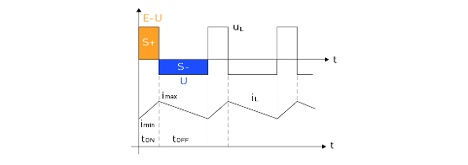
\includegraphics[width=0.75\textwidth]{Figures/Figure 2.2.png}
    \caption{The Buck Converter – Inductor Voltage and Current Versus Time Graph.}
    \label{fig:buck_waveforms1}
\end{figure}

\paragraph{Design Consideration and Calculations:}
The output voltage is determined by the duty cycle $D$:
\begin{equation}
    U = D \cdot E
\end{equation}

To limit the peak-to-peak inductor current ripple $\Delta I_L$, the minimum required inductance $L$ is governed by the switching frequency $f_s$ and the input voltage:
\begin{equation}
    L = \frac{(E - U) \cdot D}{\Delta I_L \cdot f_s}
\end{equation}

Similarly, the output filtering capacitance $C$ must mitigate the output voltage ripple $\Delta U$. The capacitance value is computed based on the allowable peak-to-peak ripple:
\begin{equation}
    C = \frac{\Delta I_L}{8 \cdot f_s \cdot \Delta U}
\end{equation}
The output capacitor plays a vital role in filtering the output voltage ripple and maintaining stability in the converter, depending directly on the intended output voltage ripple, the ripple current, and the switching frequency.

\newpage

% -------------------------------------------------------------------------
\subsubsection{Boost Converter}
The boost converter is a step-up switching topology utilized when the application demands an output voltage greater than the source input ($U > E$).

\paragraph{Circuit Diagram:}
\begin{figure}[H]
    \centering
    
\includegraphics[width=0.75\textwidth]{Figures/Figure 2.3.png}
    \caption{The Boost Converter Circuit Diagram – Interval $t_{ON}$.}
    \label{fig:buck_waveforms}
\end{figure}

\begin{figure}[H]
    \centering
    
\includegraphics[width=0.75\textwidth]{Figures/Figure 2.4.png}
    \caption{The Boost Converter Circuit Diagram – Interval $t_{OFF}$.}
    \label{fig:buck_waveformss}
\end{figure}

\paragraph{Introduction and Principle of Operation:}
Boost converters efficiently step up an input voltage to a higher output voltage by storing energy in an inductor during the switch-on phase and releasing it to the load during the switch-off phase. Power electronics applications requiring a greater output voltage than the input source depend heavily on this topology. The operational stages are broken down as follows:

\begin{itemize}
    \item \textbf{Switch-on period ($S$ closed, diode reverse biased):} Switch S is closed, shorting the right side of the inductor directly to the return path. Diode D is reverse-biased by the output voltage U, isolating the load stage. The input voltage E is applied entirely across L, causing the inductor current to ramp upward linearly from $i_{min}$ to $i_{max}$, storing energy within its magnetic core.
    \begin{equation}
        u_L = E
    \end{equation}
    \begin{equation}
        \Delta I_L = \frac{E \cdot t_{ON}}{L}
    \end{equation}

    \newpage
    
    \item \textbf{Switch-off period ($S$ open, diode forward biased):} Switch S opens. To sustain current continuity, the inductor induces a positive voltage that adds in-series with the source voltage E. Diode D becomes forward-biased, dumping the combined energy of the source and the inductor into the output capacitor and load.
    \begin{equation}
        u_L = E - U
    \end{equation}
\end{itemize}

By equating the inductor current changes for both stages, the voltage conversion relationship for the boost converter yields:
\begin{equation}
    U = \frac{E}{1 - D}
\end{equation}
where $D$ is the duty cycle, defined as the ratio of the switch-on time ($t_{on}$) to the total switching period ($T$).

\begin{figure}[H]
    \centering
    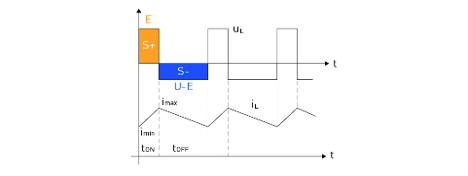
\includegraphics[width=0.75\textwidth]{Figures/Figure 2.5.png}
    \caption{The Boost Converter - Inductor Voltage and Current Versus Time Graph.}
    \label{fig:boost_waveforms}
\end{figure}

\paragraph{Design Consideration and Calculations:}
In continuous conduction mode (CCM), the duty cycle $D$ determines the voltage step-up relationship as follows:
\begin{equation}
    D = \frac{U - E}{U}
\end{equation}
This equation is valid for the continuous conduction mode (CCM) operation. The duty cycle is important for selecting the appropriate switching frequency and inductor value.
\\
\\
The average inductor current matches the average input current ($I_L = I_{in}$). The inductor value $L$ required to restrict current ripples to a target percentage is calculated using:
\begin{equation}
    L = \frac{E \cdot D}{\Delta I_L \cdot f_s}
\end{equation}

The output capacitor provides sole power to the load during the switch-on period $t_{ON}$. Therefore, to restrict the output voltage ripple $\Delta U$, the capacitance is sized as follows:
\begin{equation}
    C = \frac{I_{out} \cdot D}{\Delta U \cdot f_s}
\end{equation}



% -------------------------------------------------------------------------
\subsubsection{Interleaved Boost Converter}
When applications scale to high power levels, standard single-phase boost converters face severe limitations, including high thermal stresses on semiconductor components, large passive component footprints, and significant input current ripples. To overcome these constraints, an Interleaved Boost Converter (IBC) topology is deployed [11].

\paragraph{Circuit Diagram:}
\begin{figure}[H]
    \centering
    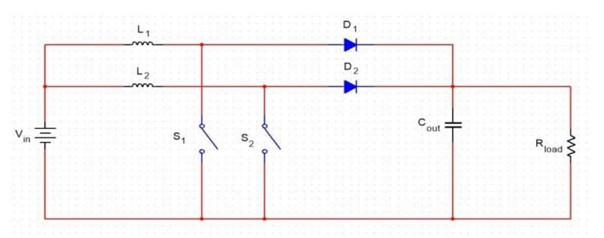
\includegraphics[width=0.75\textwidth]{Figures/Figure 2.6.jpg}
    \caption{Interleaved DC-DC Boost Converter Circuit Diagram.}
    \label{fig:ibc_circuit}
\end{figure}

\paragraph{Introduction and Principle of Operation:}
The multiphase interleaved configuration splits the power path into parallel branches ($N$ phases). For a standard two-phase interleaved system, two identical boost branches operate at the same switching frequency $f_s$, but their gate drive signals are intentionally phase-shifted by $180^\circ$ ($\frac{360^\circ}{N}$) [11].

Because the inductor ripple currents $i_1$ and $i_2$ are out of phase, their ripples structurally cancel each other out when summing at the input node, effectively doubling the apparent ripple frequency to $2f_s$ [11].

The two-phase IBC steps through four discrete operating modes based on the overlapping states of switches $S_1$ and $S_2$:
\begin{itemize}
    \item \textbf{Mode 1 ($S_1$ ON, $S_2$ ON):} Both switches are closed and diodes $D_1$ and $D_2$ are reverse-biased. Both inductors $L_1$ and $L_2$ absorb energy simultaneously from the input source $V_{in}$, with both currents rising linearly. The output load is supported entirely by the filtering capacitor $C_{out}$.
    \begin{figure}[H]
    \centering
    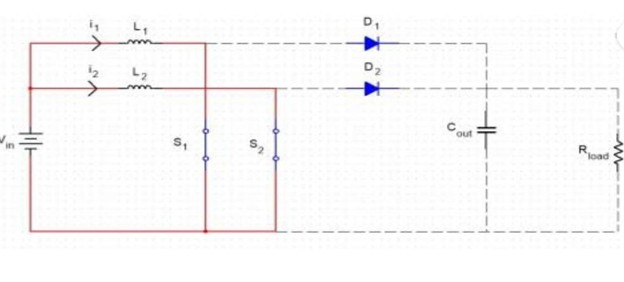
\includegraphics[width=0.65\textwidth]{Figures/Figure 2.7.jpg}
    \caption{Mode 1.}
    \label{fig:ibc_circuit2}
\end{figure}
    \item \textbf{Mode 2 ($S_1$ ON, $S_2$ OFF):} Switch $S_1$ remains closed, continuing to charge $L_1$, while switch $S_2$ opens, forcing diode $D_2$ into conduction. Inductor $L_2$ enters its discharge phase, transferring its stored energy along with the source to the output stage.
    \begin{figure}[H]
    \centering
    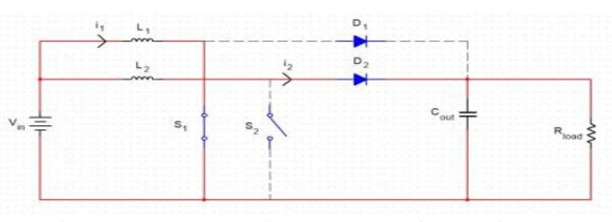
\includegraphics[width=0.75\textwidth]{Figures/Figure 2.8.jpg}
    \caption{Mode 2.}
    \label{fig:ibc_circuit22}
\end{figure}
    \item \textbf{Mode 3 ($S_1$ OFF, $S_2$ ON):} Switch $S_1$ opens, forward-biasing $D_1$, which allows $L_1$ to discharge its accumulated energy into the load. Simultaneously, $S_2$ is closed, placing $L_2$ back into its charging cycle.
    \begin{figure}[H]
    \centering
    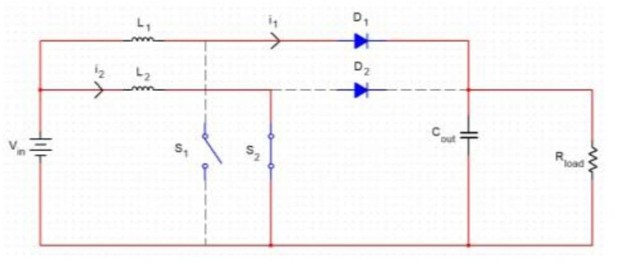
\includegraphics[width=0.75\textwidth]{Figures/Figure 2.9.jpg}
    \caption{Mode 3.}
    \label{fig:ibc_circuit3}
\end{figure}
    \item \textbf{Mode 4 ($S_1$ OFF, $S_2$ OFF):} Both switches are open (occurring when the operating duty cycle $D < 0.5$). Diodes $D_1$ and $D_2$ are forward-biased, causing both inductors to simultaneously discharge their energy into the output network.
\end{itemize}
\begin{figure}[H]
    \centering
    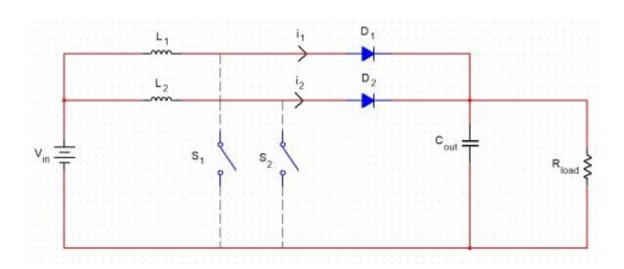
\includegraphics[width=0.75\textwidth]{Figures/Figure 2.10.jpg}
    \caption{Mode 4.}
    \label{fig:ibc_circuit4}
\end{figure}

\paragraph{Design Consideration and Calculations:}
The conversion duty cycle equation mirrors the conventional boost setup:
\begin{equation}
    D = \frac{V_{out} - V_{in}}{V_{out}}
\end{equation}
The total average input current is split equally among the $N=2$ phases:
\begin{equation}
    I_L = \frac{I_{in}}{2}
\end{equation}
Each phase inductor is sized independently using the single-phase ripple requirements:
\begin{equation}
    L_1 = L_2 = \frac{V_{in} \cdot D}{\Delta I_{L\_phase} \cdot f_s}
\end{equation}
The output filtering capacitance value is computed via:
\begin{equation}
    C_{out} = \frac{I_{out} \cdot D}{\Delta V_{out} \cdot f_s}
\end{equation}

So, Whenever high power, and high voltage gains are desired, single stage conventional boost converters are not sufficient as they produce high voltage and current ripples, increased switching stress and low conversion efficiency.
Interleaving technology in this regard can prove effective to meet these requirements with the benefits of the following [11];
\\
\\
-High voltage gain.
\\
-Input current ripple elimination and low conduction losses.
\\
-Reduced ripple output voltage.
\\
-Low voltage stress on switches.

% -------------------------------------------------------------------------
\subsubsection{Two-Quadrant Chopper}
The basic architecture consists of two fully controlled semiconductor switches $S_1, S_2$ connected in series across the primary DC link, with anti-parallel freewheeling diodes ($D_1, D_2$) paired across each switch. The load network is characterized by an inductive-resistive filter acting in series with a secondary voltage source $E_{load}$.

\paragraph{Circuit Diagram:}
\begin{figure}[H]
    \centering
    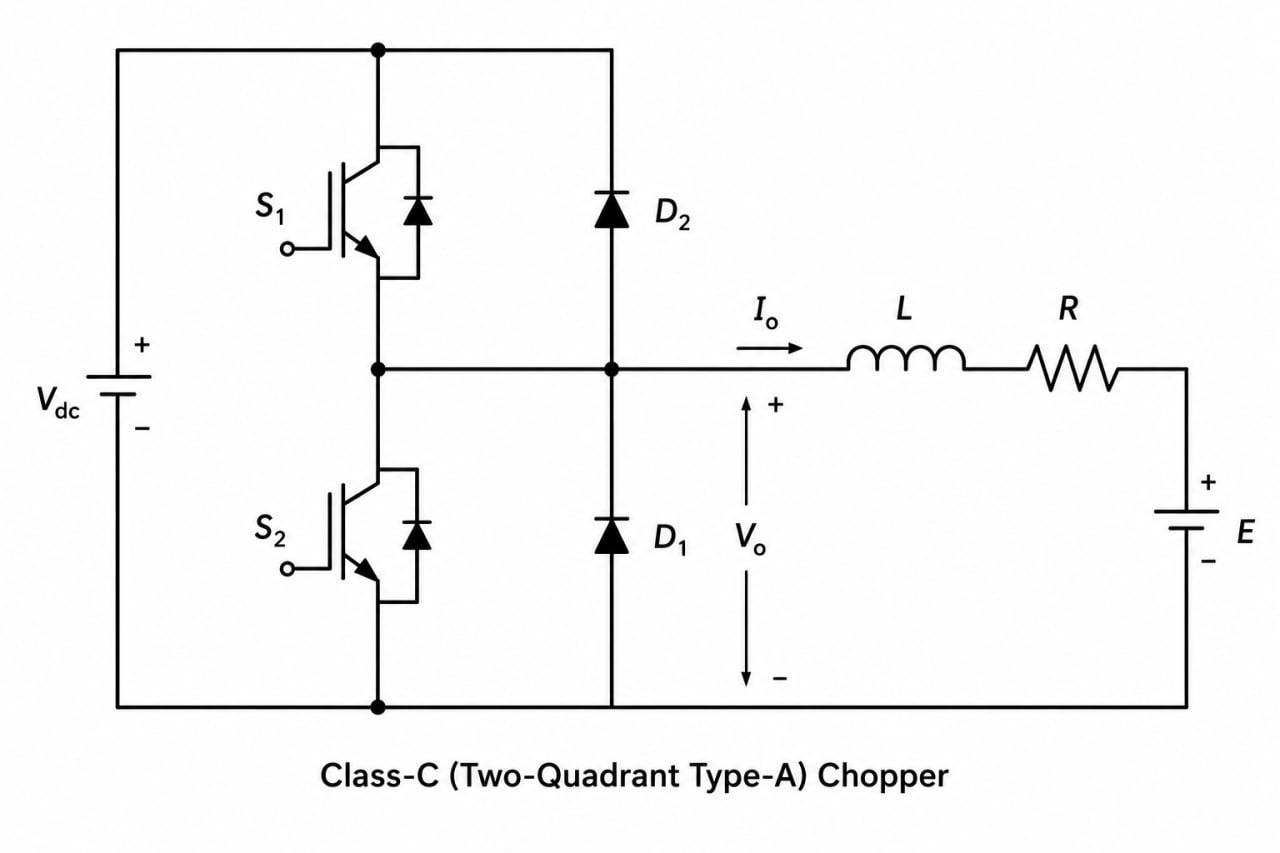
\includegraphics[width=0.5\textwidth]{Figures/Figure 2.11.jpg}
    \caption{Two Quadrant Chopper Circuit Diagram.}
    \label{fig:two_quad_circuit}
\end{figure}

\paragraph{Introduction and Principle of Operation:}
A Class-C chopper is a two-quadrant chopper operating in the first and second quadrants of the output voltage and current plane. Structurally, it represents a parallel combination of Class-A (step-down) and Class-B (step-up) choppers arranged in a complementary half-bridge configuration. This configuration allows for reversible power flow while maintaining a unipolar positive output voltage polarity. To prevent destructive shoot-through faults across the DC link, the gate drive signals for $S_1$ and $S_2$ must be mutually exclusive with an integrated dead-time interval.

\begin{itemize}
    \item \textbf{First Quadrant Operation (Forward Power Flow / Buck Mode):} Both $V_O$ and $I_o$ must remain positive, channeling power from the source $V_{dc}$ to the load.
    \begin{itemize}
        \item \textit{Interval 1 ($S_1$ ON, $S_2$ OFF):} When switch $S_1$ is active, the load is tied directly to the input source ($V_O = V_{dc}$), causing the inductor to store magnetic energy forwardly.
        \item \textit{Interval 2 ($S_1$ OFF, $S_2$ OFF):} When $S_1$ turns off, the inductor forward-biases freewheeling diode $D_1$. The current decays linearly through $D_1$ in the forward direction, forcing terminal voltage down to zero ($V_O = 0$).
    \end{itemize}
    
    \begin{figure}[H]
    \centering
    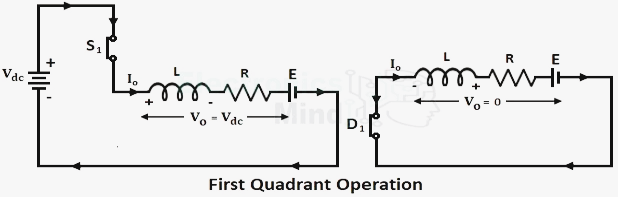
\includegraphics[width=0.55\textwidth]{Figures/Figure 2.12.png}
    \caption{Two Quadrant Chopper First Quadrant Operation.}
    \label{fig:two_quad_circuit2}
\end{figure}
    
    \item \textbf{Second Quadrant Operation (Reverse Power Flow / Boost Mode):} Terminal voltage $V_O$ remains positive, but the load current reverses direction ($-I_o$), requiring the active load source $E_{load}$ to drive energy back into the primary supply.
    \begin{itemize}
        \item \textit{Interval 1 ($S_2$ ON, $S_1$ OFF):} Switch $S_2$ turns on, short-circuiting the loop containing the inductor, load resistance, and active source $E_{load}$ ($V_O = 0$), storing energy inside the inductor negatively.
        \item \textit{Interval 2 ($S_2$ OFF, $S_1$ OFF):} When $S_2$ opens, the inductor's magnetic field collapses and forces diode $D_2$ into conduction, discharging energy back into the main supply link ($V_O = V_{dc}$).
    \end{itemize}
\end{itemize}

\begin{figure}[H]
    \centering
    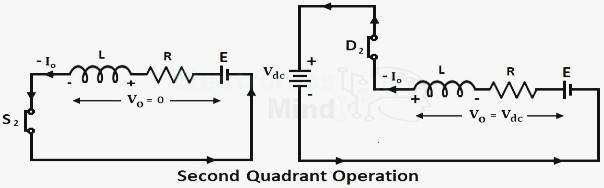
\includegraphics[width=0.55\textwidth]{Figures/Figure 2.13.jpg}
    \caption{Two Quadrant Chopper Second Quadrant Operation.}
    \label{fig:two_quad_circuit3}
\end{figure}

The continuous conduction mode transitions through four specific semiconductor states: $V_O=V_{dc}$ and $I_o>0$ (S1 conducting); $V_O=0$ and $I_o>0$ (D1 conducting); $V_O=0$ and $I_o<0$ (S2 conducting); and $V_O=V_{dc}$ and $I_o<0$ (D2 conducting).

\begin{figure}[H]
    \centering
    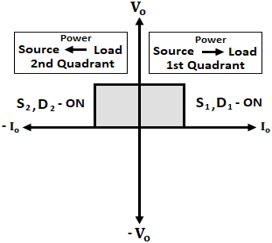
\includegraphics[width=0.55\textwidth]{Figures/Figure 2.14.png}
    \caption{Two Quadrant Operation.}
    \label{fig:two_quad_circuit4}
\end{figure}

Therefore, the output voltage $V_O = +V_{dc}$ (i.e., $V_O$ is positive) when $S_1$ or $D_2$ conducts, and $V_O$ is zero when $D_1$ or $S_2$ conducts. The output current $I_o$ is positive when $S_1$ or $D_1$ conducts, and $I_o$ is negative when $S_2$ or $D_2$ conducts. 
The waveforms of the Class-C chopper are illustrated below:

\begin{figure}[H]
    \centering
    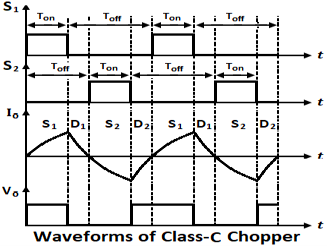
\includegraphics[width=0.6\textwidth]{Figures/Figure 2.15.png}
    \caption{Two-Quadrant Chopper Waveforms.}
    \label{fig:two_quad_waveforms}
\end{figure}

\newpage

In the above waveforms, when $S_1$ is ON, $I_o$ increases gradually to its maximum value and $V_O$ is positive. When $S_1$ is OFF, $V_O$ becomes zero and $I_o$ decreases gradually through $D_1$, which represents the discharge current of the inductor in the forward direction. When $S_2$ is ON, $V_O$ remains zero and $I_o$ increases negatively due to current flow in the reverse direction. When $S_2$ is OFF, $V_O$ becomes positive and $I_o$ decreases gradually from its negative maximum through $D_2$, which represents the discharge current of the inductor in the reverse direction.

The continuous conduction mode transitions through four specific semiconductor conduction states over a complete switching cycle:
\begin{itemize}
    \item $V_O = V_{dc}$ and $I_o > 0$ when $S_1$ is conducting.
    \item $V_O = 0$ and $I_o > 0$ when $D_1$ is conducting.
    \item $V_O = 0$ and $I_o < 0$ when $S_2$ is conducting.
    \item $V_O = V_{dc}$ and $I_o < 0$ when $D_2$ is conducting.
\end{itemize}

Since the output voltage is always positive and the output current can be either positive or negative, this topology represents a reversible power flow. Power flows from the source to the load when the chopper operates in the first quadrant, whereas power flows from the load back to the source when the chopper operates in the second quadrant. Additionally, extreme care must be taken to ensure that both switches are never turned ON at the same time, as this results in a catastrophic cross-conduction (shoot-through) short-circuit across the DC supply source.

\paragraph{Design Consideration and Calculations:}
The smoothing inductor $L$ is sized to suppress the peak-to-peak current ripple $\Delta i_L$ under the worst-case operating scenarios across both modes:
\begin{align}
    L_{buck} &= \frac{E_{load} \cdot (1 - D_{buck})}{\Delta i_L \cdot f_{sw}} \\
    L_{boost} &= \frac{V_O \cdot (V_{dc} - V_O)}{\Delta I_o \cdot f_s \cdot V_{dc}}
\end{align}
To ensure steady-state stability across both modes, the final chosen inductor value must satisfy the maximum boundary envelope:
\begin{equation}
    L_{optimal} = \max(L_{buck}, L_{boost})
\end{equation}
\newpage
\subsection{Conclusion of Converter Topologies}
\begin{itemize}
    \item \textbf{Buck Converter:} Operates strictly as a step-down regulator, ideal for down-converting voltage for low-power digital control stages, but restricted to unidirectional current delivery.
    \item \textbf{Boost Converter:} Functions exclusively as a step-up topology for low-voltage inputs, though it experiences high ripples at elevated power levels.
    \item \textbf{Interleaved Boost Converter:} Enhances the conventional setup by paralleling multi-phase branches with an explicit spatial delay ($\frac{360^\circ}{N}$), canceling out ripple currents and reducing component sizing constraints.
    \item \textbf{Two-Quadrant Chopper:} Couples step-down and step-up traits into a cohesive half-bridge structure, managing current reversibility while maintaining unipolar positive voltage to achieve seamless bidirectional transitions essential for battery energy storage systems (BESS) and electric vehicle (EV) charging stations.
\end{itemize}